\documentclass[a4paper,12pt]{article}

\usepackage{fancyhdr}						% for headers and footers.
\usepackage{setspace}						% for using single spaces.
\usepackage{mathptmx}						% for Times Roman Closest to Times New Roman.
\usepackage{listings}						% for code sections.
\usepackage{color}							% for colouring the code sections.	
\usepackage[authoryear]{natbib}			% for refrencing.

\bibliographystyle{apalike}					% set refencing style
\bibpunct{(}{)}{;}{a}{,}{,}

\hyphenpenalty 10000						% remove hyphenation at page width
\exhyphenpenalty 10000

\makeatletter								% remove Refrence Title buit into biblatex.
\renewenvironment{thebibliography}[1]{
      \list{\@biblabel{\@arabic\c@enumiv}}
           {\settowidth\labelwidth{\@biblabel{#1}}
            \leftmargin\labelwidth
            \advance\leftmargin\labelsep
            \@openbib@code
            \usecounter{enumiv}
            \let\p@enumiv\@empty
            \renewcommand\theenumiv{\@arabic\c@enumiv}}
      \sloppy
      \clubpenalty4000
      \@clubpenalty \clubpenalty
      \widowpenalty4000
      \sfcode`\.\@m}
     {\def\@noitemerr
       {\@latex@warning{Empty `thebibliography' environment}}
      \endlist}
\makeatother

\pagestyle{fancy}							% use the fancy theme.
\fancyhead{}								% clear the headers.
\fancyfoot[CE,CO]{\leftmark}				% Put the Section into the footer.
\fancyfoot[LE,RO]{\thepage}					% put the page number into the footer.
\renewcommand{\headrulewidth}{0pt}			% remove the header rule / line.
\renewcommand{\footrulewidth}{0.4pt}		% place the footer rule / line.

\definecolor{dkgreen}{rgb}{0,0.6,0}		% define colours.
\definecolor{gray}{rgb}{0.5,0.5,0.5}		
\definecolor{mauve}{rgb}{0.58,0,0.82}
\definecolor{backcolour}{rgb}{0.95,0.95,0.92}
\definecolor{numbercolour}{rgb}{0.4,0.4,0.4}

\lstset{frame=tb,							% Set up code section settings.
  language=Java,							% language is java.
  aboveskip=3mm,							% top padding text.
  belowskip=3mm,							% bottom padding between text.
  showstringspaces=true,					% remove space characters.
  columns=flexible,							% flexible columns.
  basicstyle={\small\ttfamily},			% font.
  numbers=left,								% show line numbers on the left.
  numbersep=5pt, 							% size of line numbers.
  frame = false,							% remove the frame.
  backgroundcolor=\color{backcolour}, 		% set the colours.
  numberstyle=\tiny\color{gray},
  keywordstyle=\color{blue},
  commentstyle=\color{dkgreen},
  stringstyle=\color{mauve},
  numberstyle=\color{numbercolour},
  breaklines=false,							% don't break lines.
  breakatwhitespace=false,					% allow whitespace.
  tabsize=4									% set tab size.
}

\input{glyphtounicode}						% enable unicode.
\pdfgentounicode=1
\singlespacing								% enable single spaces.

\begin{document}
	%
% The MIT License (MIT)
%
% Copyright (c) 2014 Paul Batty
%
% Permission is hereby granted, free of charge, to any person obtaining a copy
% of this software and associated documentation files (the "Software"), to deal
% in the Software without restriction, including without limitation the rights
% to use, copy, modify, merge, publish, distribute, sublicense, and/or sell
% copies of the Software, and to permit persons to whom the Software is
% furnished to do so, subject to the following conditions:
%
% The above copyright notice and this permission notice shall be included in
% all copies or substantial portions of the Software.
%
% THE SOFTWARE IS PROVIDED "AS IS", WITHOUT WARRANTY OF ANY KIND, EXPRESS OR
% IMPLIED, INCLUDING BUT NOT LIMITED TO THE WARRANTIES OF MERCHANTABILITY,
% FITNESS FOR A PARTICULAR PURPOSE AND NONINFRINGEMENT. IN NO EVENT SHALL THE
% AUTHORS OR COPYRIGHT HOLDERS BE LIABLE FOR ANY CLAIM, DAMAGES OR OTHER
% LIABILITY, WHETHER IN AN ACTION OF CONTRACT, TORT OR OTHERWISE, ARISING FROM,
% OUT OF OR IN CONNECTION WITH THE SOFTWARE OR THE USE OR OTHER DEALINGS IN
% THE SOFTWARE.
%

\begin{titlepage}
	\begin{center}
		\begin{huge}
			\textbf{SQLite Visualiser: Building a tool to visualise the SQLite file format and log all changes.}
		\end{huge}	
		
		
		\vspace{2cm}		
		
		\normalsize By:   \\
		\large Paul Batty
		
		\vspace{2.5cm}
		
		\normalsize Supervisor: \\
		\large Andrew Scott
		
		\vspace{1.5cm}
		
		\large March 2016
		
		\vfill 
		
		\normalsize
		The dissertation is submitted to \\
		Lancaster University \\
		As partial fulfilment of the requirements for the degree of \\
		Integrated Masters of Science in Computer Science \\
	\end{center} 
\end{titlepage}

	\section*{\centering Abstract}
\begin{center}
	The Abstract.
\end{center} 

	\section*{Introduction}
\label{sec:introduction}

Having studied Databases in my previous year, including SQLite. I remember that it could do so much without the need to configure, manipulate, or go through a long winded install process. It was so simple and flexible, anyone could use it. In fact SQLite takes pride that it is probably one of the most widely deployed database engines. And one of the top five most deployed software modules. Alongside zlib, libpng and libjpg. It finds itself inside all of the top browsers (Firefox, Google chrome and possibly Edge), Operating systems (Windows 10, IOS and embed OS's) and in the most unexpected places such as aircraft.
\\\\
After doing some reading and looking at the SQLite's claim to fame. I began to take a closer look at its systems. What makes it so flexible, fast and simple to use. My main focus however was on the file format that it uses to store the entire database. How it was put together. How to traverse it. And why it is the way it is. I also looked at the available tools that are currently available for SQLite. This is covered in the first section of this paper.
\\\\
Understanding the file format was just the first stepping stone, as I then undertook a journey to build a tool that could traverse and read the file. While recording every operation that was and ever will be performed to it. This is covered in the second and third chapters.
\\\\
While building by tool. I kept two things in mind. How it operated from a users perspective and the best ways to break it. This was to ensure that the tool was open to everyone, and would not fall down and crumble. This is covered in sections four. 
\\\\
Once the tool became well developed. I started looking towards the future of the tool. What could be added to make it ever more useful for developers, researchers and anyone else using SQLite systems. This is covered in the final sections, five and six.
\\\\
The main aim of this paper is to help you understand the SQLite file format and systems. While providing a useful tool that can help debug, manipulate and record your own SQLite databases, without the need for a hex editor.

	\section{Background}
\label{sec:background}

\subsection{The Problem}
\label{subsec:the_problem}

Throughout Sqlite's history many tests, papers, and tools have been developed in order to understand, and modify the future direction of Sqlite. However, when a user wants to understand at a deeper level how Sqlite is working or finding obscure bugs, they are stuck with manually trawling through a Hex editor. This paper aims to solve this by providing a visualisation of the internal structure, as well as a update log that is updated in real time, when the database is modified.


\subsection{Sqlite}
\label{subsec:sqlite}

\subsubsection{What is Sqlite}
\label{subsubsec:what_is_sqlite}

Sqlite is a single self-contained, serverless SQL database engine. Started on 29 May 2000 by D. Richard Hipp \citep{sqlite} from gathered inspiration while working on software for guided missiles on a battleship where they needed a self-contained portable database. \citep{sqlitedefguide} He joined up with Joe Mistachkin followed by Dan Kennedy in 2002. Version 1.0 was released in August 2000, then in just over year on the 28 November 2001 2.0 which introduced, brining the BTrees and many of the features seen in 3.0. Which came a lot later containing a full rewrite and improvement over 2.0, with the first public release on 18 June 2004. At the time of writing this paper we are currently sitting at version 3.10.4 \citep{sqlite}.
\\\\
Sqlite is open source within the public domain making it accessible to everyone. The entire library size can be 350Kib, with some option features omitted it could be reduced to around 300Kib making it incredibly small compared to what it does. In addition to this the runtime usage is minimal with 4Kib stack space and 100Kib heap, allowing it to run on almost anything. Sqlite's main strength is that the entire database in encoded into a single portable file, that can be read, on any system whether 32 or 64 bit, big or small endian. It is often seen as a replacement for storage files rather then a database system \citep{sqlite}.

\subsubsection{Where is Sqlite used}
\label{subsubsec:where_is_sqlite}

Sqlite is used...


\subsection{The Sqlite file format}
\label{subsec:sqlite_file_format}

\subsubsection{The page system}
\label{subsubsec:sqlite_page_system}

Sqlite is made up of pages..

\subsubsection{The Trees and Cells}
\label{subsubsec:sqlite_trees_and_cells}

The Trees and cells...

\subsubsection{Encoding of the data}
\label{subsubsec:sqlite_data_encoding}

The Data is...

\subsection{Similar Programs}
\label{subsec:similar_programs}

\subsubsection{Sqlite browser}
\label{subsubsec:sqlite_browser}

One Similar program...
	\section{Design}
\label{sec:design}

In this section I go over the high level overview of my applications design. Starting with the high level, and going into more depth looking at each module.

\subsection{Features}
\label{subsec:Features}
As mentioned in the last section, I wanted a cross platform tool, that would enable anyone to view the internal structure of a SQLite database. With consistency and reliability. The application comes with five main features, all building upon one feature.  
\\\\
The central feature is the visualiser. The visualiser allows you to see the broken down page structure and hierarchy. So you can see how you SQLite database is laved out. On top of this you can click a node in order to see more information about. Such as data, page number e.t.c
\\\\
In addition to the visualiser, there is also a meta data tab, that will allow you to view, the header information in the database. Alongside other statistics that come from parsing the database. Such as number of tables, primary keys and so on.
\\\\
The last main feature ties into the base feature, that allows real time updating of this data when any command from any system modifies the database in some way shape or form. The live updating allows you to step through the time line of updates that have occurs while the application is running. You can also pause it if you want to inspect a certain state. 
\\\\
Whenever a update occurs, all changes that happened are recorded inside a log, and a "snapshot" of the database is taken. This snapshot is then presented to use, through the visualiser, metadata and log tabs. Creating the time line that you can then browse. 
\\\\
Apart from just showing you data, you can also execute SQL onto the database, through the SQL executor and view the schema and tables currently inside the database.

\subsection{High level Overview}
\label{subsec:high_level_overview}

From the start I wanted to build a system, that was modular and self-contained. However, as the project went on a few adjust had to my original design. When I ran into some implementation problems discussed in the next chapter. The figure~\ref{fig:design_old} shows the original design.

\begin{figure}[H]
	\centering
	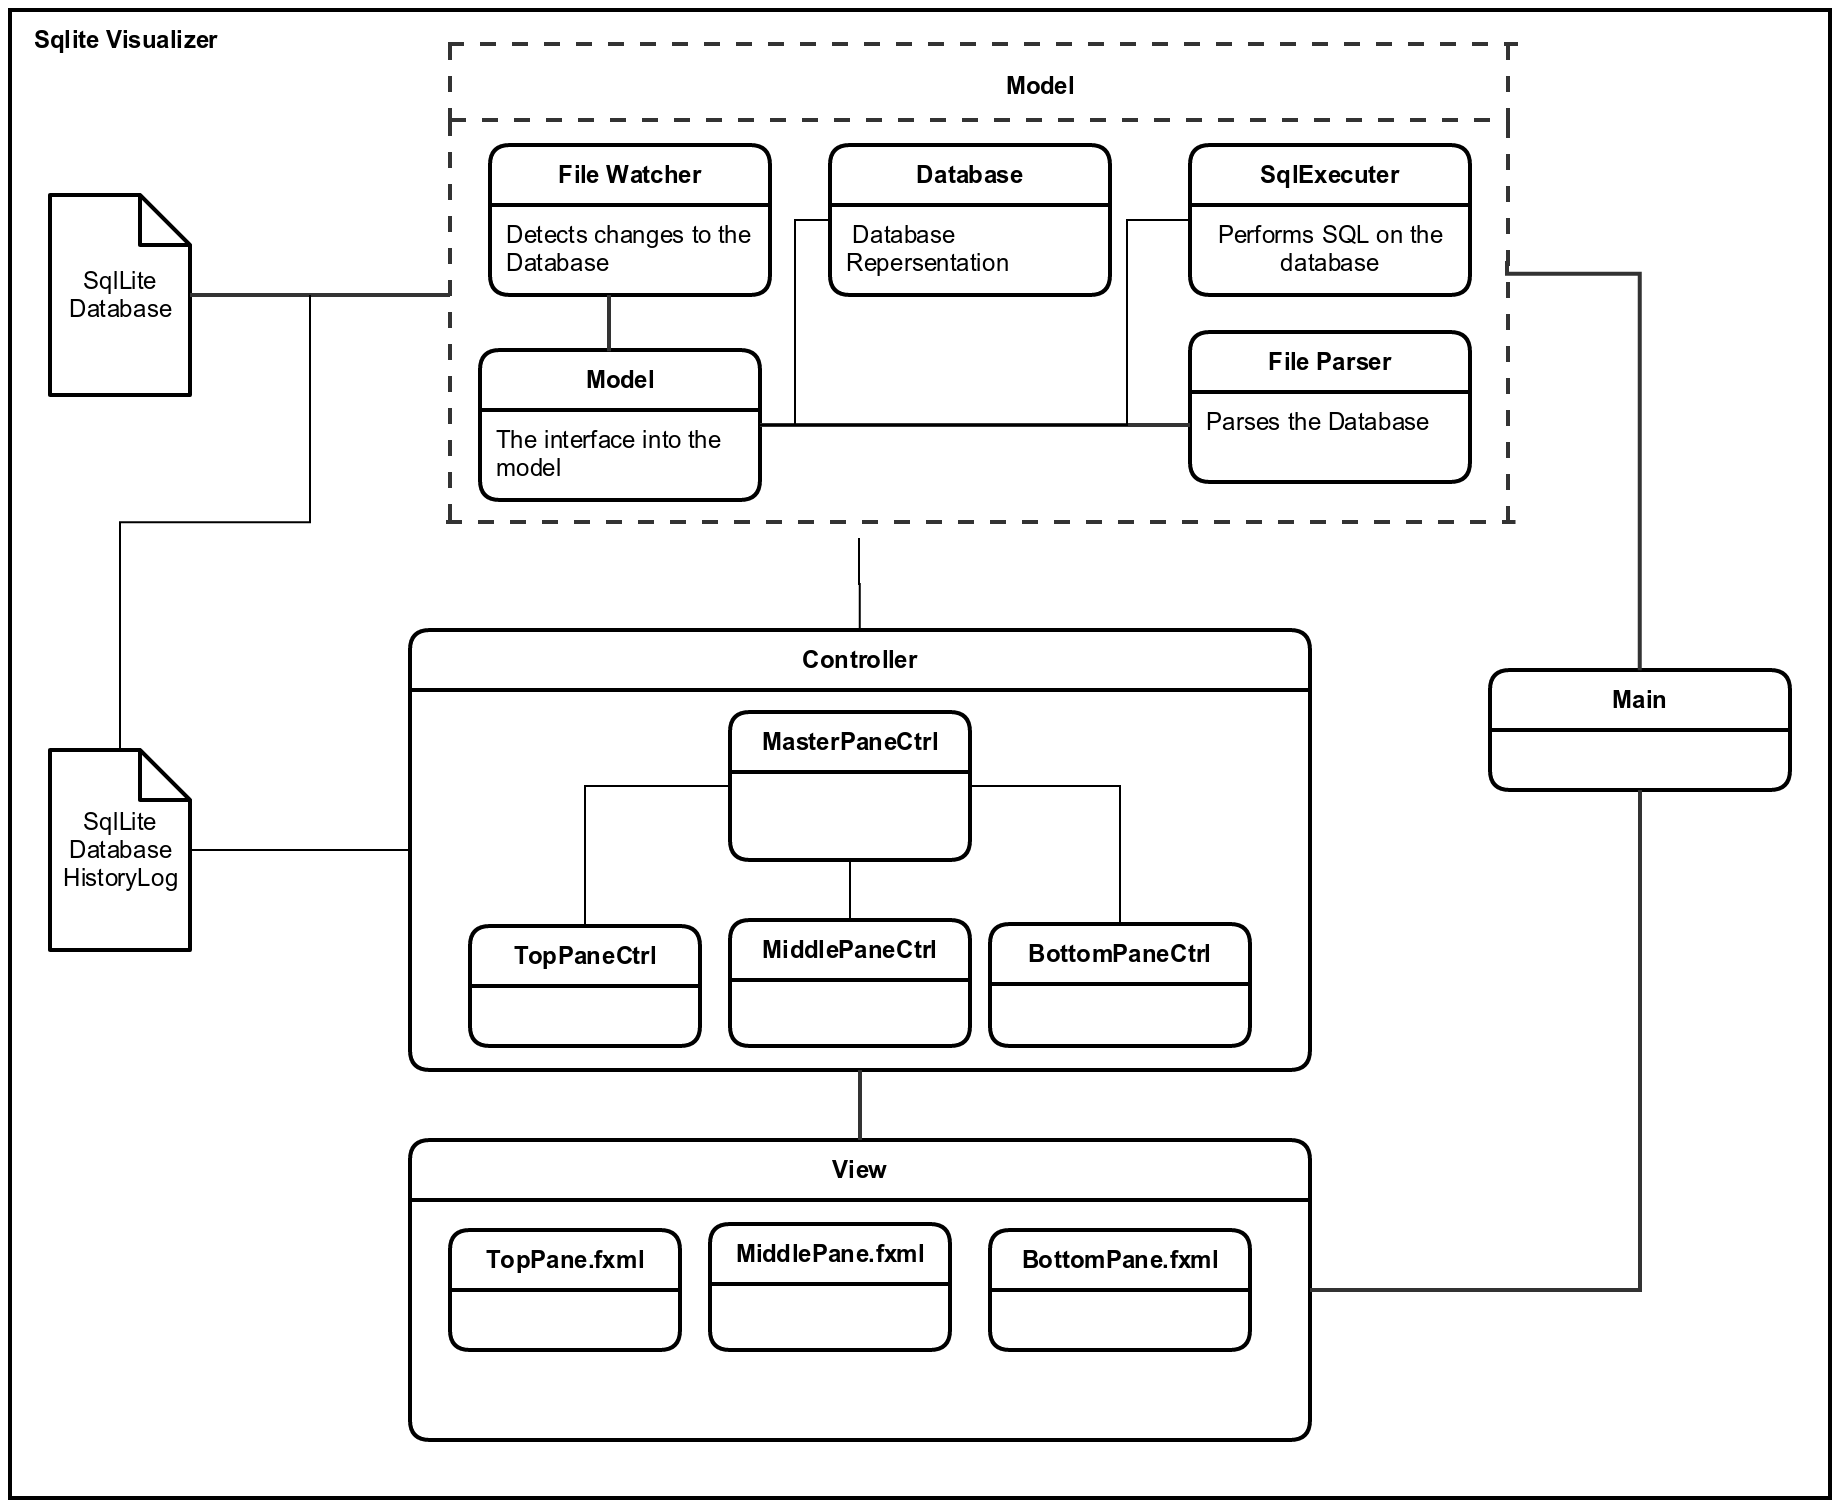
\includegraphics[scale=0.2]{images/system_diagram_old.png}
	\caption{Original system diagram}
	\label{fig:design_old}
\end{figure}

As you can see, the design utilizes the MVC (Model-View-Controller) style architect in order to separate the interface from the data. This means the view will make requests to the controller, who will then in turn contact the model for information, then sending the information to be presented by the view. The idea being that the view could be switched or adjusted at anytime without breaking the application. an example of MVC can be seen below in figure~\ref{fig:mvc}.

\begin{figure}[H]
	\centering
	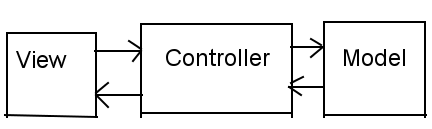
\includegraphics[scale=0.5]{images/mvc.png}
	\caption{MVC architecture}
	\label{fig:mvc}
\end{figure}

The Model was going to run in its own thread so it could control, manage and prepare the data as it came in. This meant the view could request it when it wanted. One other thing to note, is the command logging was going to store them in to an external file, for the view. However, this design proved unusable and thus changed into the following seen in figure~\ref{fig:design_new}. 

\begin{figure}[H]
	\centering
	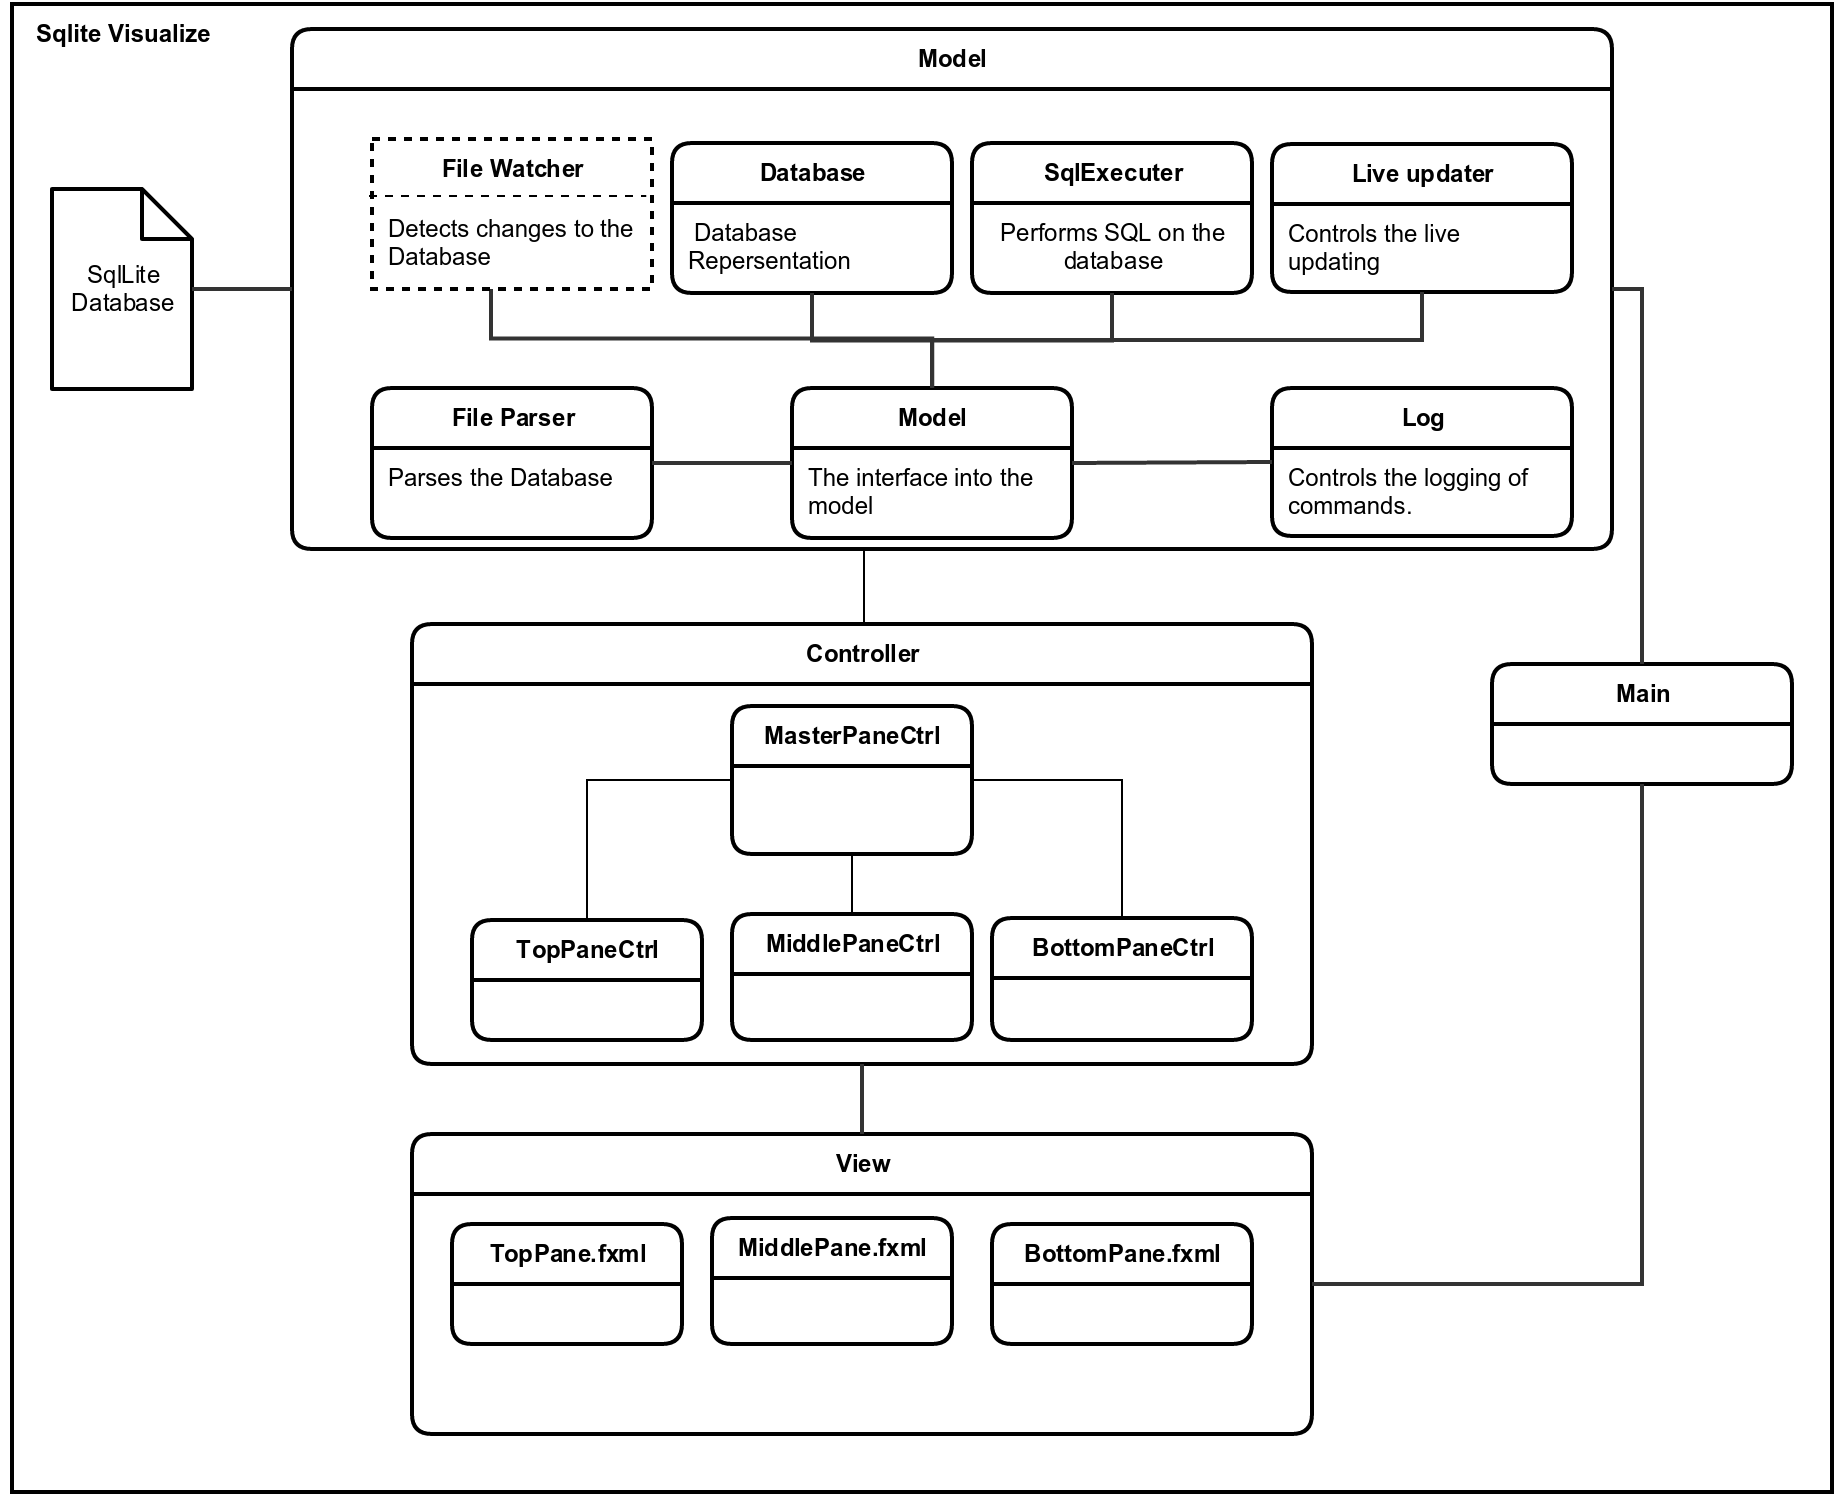
\includegraphics[scale=0.2]{images/system_diagram_new.png}
	\caption{Final system diagram}
	\label{fig:design_new}
\end{figure}

Most of the changes are seen within the Model, with the addition of two new modules. And rather then running the whole thing inside a new thread only the file watcher is. On top of this the command logging is no longer written out to file. The final change is the reduction in the amount of controllers. I will go over each of the modules in the next part.

\subsection{Module Overview}
\label{subsec:module_overview}

\subsubsection{The Main}
\label{subsubsec:main}

The main module represent the staring point of the application, it serves no other purpose other then to correctly initialise the view, model and controllers.

\subsubsection{The View}
\label{subsubsec:the_view}

The view, consists of three parts, the top, middle and right side. Since it follows the MVC style, these only contain the layout of each of the corresponding sections. The middle section however, changes depending on what is being viewed.

\subsubsection{The Controller}
\label{subsubsec:the_controller}

The controller is made up of two parts, the master controller, and the pane controller. The pane controller is changed depending on what is being viewed. Similar to the views middle pane. The master controller coordinates what is being shown. Both of them communicate to the model to collect updates, and interact with the data.

\subsubsection{The Model}
\label{subsubsec:the_model}

The model is the most complicated section and is made up of seven modules. The model itself acts as a repository design with everything connecting and interacting though it.
\\\\
All contact with the model will go though the model interface. This allows the controllers to communicate to the individual modules. In addition to this, it provides a small amount of functionality for setting up and closing. Such as opening the database. Since every module will require something from this action, the model interface will take care of setting up each module. And on exit making sure all threads have been stopped, and any other connections have been closed.
\\\\
The Database, is the in program mapping of the SQLite database system. The database is made up of two parts, the data objects, and the interface into the data object. The data object are the mapping of the SQLite database. Containing the B-Tree system, and the data. The interface provides access to the history, allowing to program move along the database time line. And management of the data objects.
\\\\
The file watcher, runs in its own thread, and utilises the observer pattern. It runs in a continuous loop waiting for a modification to happen on the database. Once a change is detect it sends a signal out over the observers, so the change is recorded. Although, if they did not tune in to the observer, the rest of the program would not receive database updates.
\\\\
The File parser, parses any given valid database file. Converting it into the database object.
\\\\
The log, takes any two database objects and records the changes between them.
\\\\
The live updater, acts like a master controller for the modules, apart from the SQL executor, file watcher and model interface. It controls what happens when a change is detected, and as such is registered to the file watchers observer. When a change is detected, the first thing it does is contact the file parser for the updated database object, send it off to the log, to record changes, and then stores it in the database module. As it controls what happens and when it can also not update, allowing the parsing to pause.
\\\\
The SQL executor, controls the SQL connections, and executes SQL commands onto the database.

\subsection{The User interface}
\label{subsec:high_user_interface}

The user interface is designed to be simplistic and easy to use. 
	%
% The MIT License (MIT)
%
% Copyright (c) 2016 Paul Batty
%
% Permission is hereby granted, free of charge, to any person obtaining a copy
% of this software and associated documentation files (the "Software"), to deal
% in the Software without restriction, including without limitation the rights
% to use, copy, modify, merge, publish, distribute, sublicense, and/or sell
% copies of the Software, and to permit persons to whom the Software is
% furnished to do so, subject to the following conditions:
%
% The above copyright notice and this permission notice shall be included in
% all copies or substantial portions of the Software.
%
% THE SOFTWARE IS PROVIDED "AS IS", WITHOUT WARRANTY OF ANY KIND, EXPRESS OR
% IMPLIED, INCLUDING BUT NOT LIMITED TO THE WARRANTIES OF MERCHANTABILITY,
% FITNESS FOR A PARTICULAR PURPOSE AND NONINFRINGEMENT. IN NO EVENT SHALL THE
% AUTHORS OR COPYRIGHT HOLDERS BE LIABLE FOR ANY CLAIM, DAMAGES OR OTHER
% LIABILITY, WHETHER IN AN ACTION OF CONTRACT, TORT OR OTHERWISE, ARISING FROM,
% OUT OF OR IN CONNECTION WITH THE SOFTWARE OR THE USE OR OTHER DEALINGS IN
% THE SOFTWARE.
%

\section{Implementation}
\label{sec:implementation}

Having looked at the overall architecture of the application, and how it is build up. This section will go over the tools used during development, how the features were implemented and the problems encountered along the way.

\subsection{The tools}
\label{subsec:the_tools}

For this particular application the programming language of choice was Java and JavaFX for the user interface and controllers. This meant right from the start the application had cross platform support. A MVC style architecture and with JDBC open access to SQL database connections. The only major issue was speed, as SQLite is known to be fast, whether the application could keep up with the requests that where being performed. However, as SQLite only allows one writer at a time this was never an issue. The other downside to using Java was not having direct access to the SQLite API through its own interface, But, after looking at the interface everything was needed is supported through JDBC.

\subsection{The Modules}
\label{subsec:the_modules}

\subsubsection{The view and controllers}
\label{subsubsec:imp_veiw}

As previously mentioned, the architecture is MVC with JavaFX and Java. JavaFX comes with a whole host of tools for working with the view, and controllers. 
\\\\
Firstly, each view or section can be represented using an FXML file. The FXML file is heavily based on HTML, including the support for CSS styling. Each file starts with a root node, normally one of the panes, such as border, anchor, and grid. For this application the majority of FXML files started with anchor panes, apart from the menu bar which used a border pane. Then following the root pane is the items to attached to it. Each item can be given a unique identifier that allows it to be controlled with via Java and CSS. In addition to this custom items can be included for use within JavaFX.
\\\\
Secondly, the controller is a normal Java class set as the controller for a particular FXML file. This can be done in two ways. The first way is to inject the controller into the loading process. This allows the application to call other methods in side the controller, such as initialisation before the FXML file is loaded. It also gives more control over the controller, and where it is used. The second way is to specify the controller inside the FXML file, and Java will load the controller in when the file is loaded. But the access to the controller object is lost. Inside the controller the annotation @FXML, allows Java to inject the item from the controller into the view, and vice versa. Giving full control over the FXML file and the object utilising the items unique identifier. Throughout this application  the first method of loading the controllers were used, to allow controller sharing, and manual control over the controller. 
\\\\
The view is made up of four sections, the menu bar, containing the file, edit and other drop downs, including the icons, and tabs. The other three section, represent the left, middle, and right sections of the central pane. This means that any one time three different views can be displayed. Each of the sections have their own FXML file, depending on the situation they may also share a controller. This can be seen below in figure~\ref{fig:view_breakdown}.

\begin{figure}[H]
	\centering
	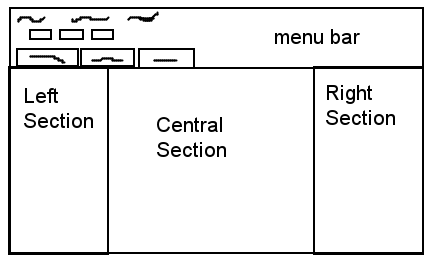
\includegraphics[scale=0.5]{images/view_breakdown.png}
	\caption{View breakdown}
	\label{fig:view_breakdown}
\end{figure}

As mentioned earlier that the menu bar will never change, and should never change. Using this fact the menu bar controller also doubles up as a `master' controller. It controls what is currently seen in the other three sections. Loading and freeing up the necessary sections for that tab. 
\\\\
The central pane is a split pane, with two split dividers allowing each sections size to be adjusted on the fly to fit the user's needs. If a section is not needed it is just a matter of hiding that panes divider bar. 
\\\\
The controllers for each section extend a abstract controller class. The controller class, enforces a model interface object into the constructor, and implements observer. The model interface allows each controller to separately contact the model, as previously mentioned to collect the data for the view. By implementing observer the controller can then be registered for the signal when the database is updated within the live updater (section~\ref{subsubsec:the_model}). Meaning that the updated information can be collected as soon as it is ready, without having to wait, or having a manual refresh button.    

\subsubsection{Model interface}
\label{subsubsec:imp_model_interface}

The model interface is based on a repository design with all the sub modules attached to it. In order for the controller to communicate with the sub modules they must also first go through the model interface. This design helps keep everything separated and compact. All of the sub modules attached to the model interface implement their corresponding interface. Allowing the implementation to change while keeping the same external view. This enables the design to be adapted to other systems other than SQLite. Below figure~\ref{fig:model_interface_design} shows the layout of the model interface.

\begin{figure}[H]
	\centering
	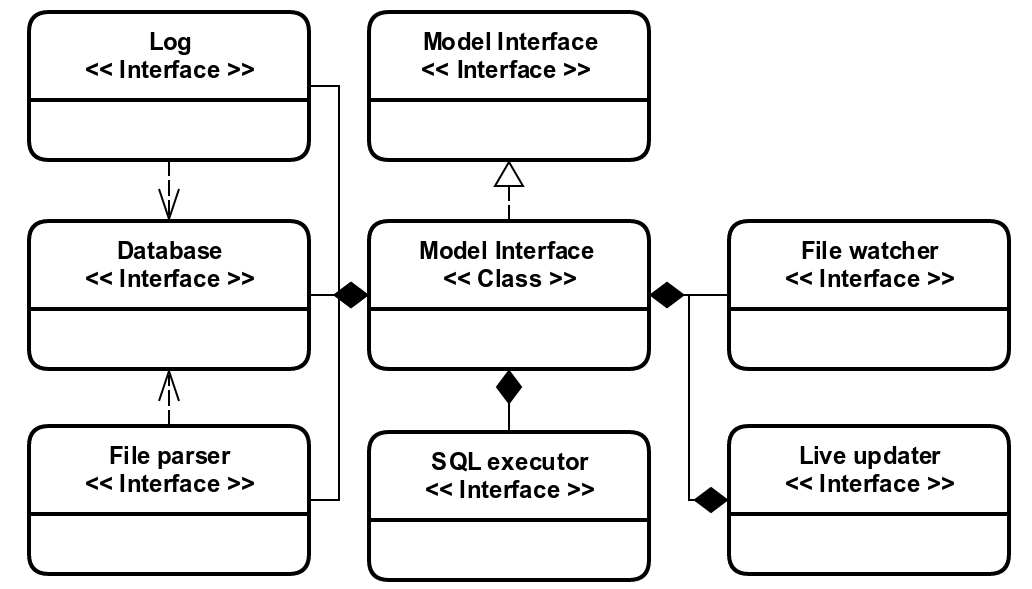
\includegraphics[scale=0.3]{images/model_interface_design.png}
	\caption{Model interface}
	\label{fig:model_interface_design}
\end{figure}

Everything is attached to the model interface, apart from the live updater being the exception with a copy of the model. In addition to providing access to the other modules, it has a very small amount of implementation, that is only used when every module is affected. Such as the case of setting up, closing and opening a database, which are all calls to the corresponding method on the modules interfaces. 

\subsubsection{The database}
\label{subsubsec:databse_imp}

The database module is made up of two parts, the interface and the storage. The interface controls access to the storage. Allowing the adding of new database items, retrieving of database items and stepping through the time line of database objects, and complete clearing of database items. Used with setting up and opening a new database, in order to make sure that the items are not mixed up with different files. The items are stored within an ArrayList, and an int counter is used to keep track of where in the array the application currently is.
\\\\
The storage is made up of database items that contain a ``snapshot" of the current state of the database file, the database item is made of two parts, the meta-data, and B-Tree. The meta-data contains all the information in the header, including a few others such as the number of tables, the file name, and page number. The B-Tree is a custom implementation, holding the various B-Tree pages as represented in the file. The database items are filled with information via the file parser. Out of all the classes, the database items are the most used, being sent to the view for displaying, and modified by the various other modules during creation. 

\subsubsection{File watcher}
\label{subsubsec:file_watcher_imp}

There were two different options available in order to detect when the database was updated. Firstly, using SQLite's API provided by SQLite to detect the changes. However, the API works on a per connection basis, meaning that the signals would only be sent along the same connection that the request came from, which are of no use, since the application knows when a command is sent. Alternatively, the application could watch the file for modifications. Since SQLite is a single file, every time the file / database is updated the last modified time would also change. In addition to this as SQLite only allows one writer at a time, this would allow the application to revive a signal every update consistently.  
\\\\
The original implementation utilised Java's WatchService API. However, during use it tended to be hit or miss whether it would register the change. At one point it failed to detect any changes. In the end a custom solution had to be made, using a simple while true loop, recording the last modified time, then when the time differs it sends out a single to the rest of the application. 
\\\\
Due to the polling nature of this module, it runs inside its own thread, and communicates over an observer pattern, that any another class can tune into, providing they implement the Observer interface. The thread could then process the updated databases without stopping or slowing down the user interface and other interactions.
\\\\
The final implementation, effectively detected all changes performed to the database consistently. Since it was custom made it was also a lot lighter than the other alternatives. In addition to this the loop had no performance hit on the computation or the rest of the application.

\subsubsection{File parser}
\label{subsubsec:file_parser_imp}

The file parser takes a database file, a database object, and converts the database file into the database object. Parsing the database, starts with checking the magic number, then the header, before moving onto the pages. The magic number and header information is correctly reading the first 100 bytes of the file, See Appendix A for the header layout. To parse the pages the application heavily relied upon recursion.
\\\\
First it would parse the page header, then switch into the method, that dealt with that type of page, who would then call the original method, when it reached a page number.  Each page was represented as a node, with contents of the node represented as a cell. The only main issue with this design is the size of the stack on a large database. Below is the psudocode of the algorithm:

\begin{lstlisting}	
public void parseBTree(stream, database) {
	database.getBTree().setRoot(parsePage(stream, 1, 
								database.getPageSize()));
}

public Node parsePage(stream, pageNumber, pageSize) {
	Node node = new Node();
	PageHeader header = parseHeader(stream, pageNumber, pageSize);
	
	BTreeCell cell;
	switch(header.getType()) {
		case (TABLE_BTREE_LEAF_CELL) {
			cell = parseTableBtreeLeafCell(stream, pageNumber, 
											pageSize);
		}
		....
	}
	if (header.getType() == INTERIOR_CELL) {
		node.addChild(parsePage(in, pageHeader.getRightMostPointer(), 
						pageSize));
	}
	node.setData(cell);
	return node;
}

public cell parseTableBtreeLeafCell(InputStream, PageHeader, Node) {
	Cell cell = new Cell();
	
	int cellPointers[] = header.getCellPointers();
	foreach(cellpointer) {
		cell.data = readData();		
		if (cell has pageNumber) {
			node.addChild(parsePage(in, pagenumber, 
						pageSize));
		}
	}
	
	return cell;
}
\end{lstlisting}

During the process of parsing the tree the file parser will also need to decode the `varints' mentioned in section~\ref{subsubsec:sqlite_data_encoding} especially as they are needed to count the number of bytes for the record headers. Below shows the psudocode algorithm that decrypts them, to both retrieve the encrypted number and the number of bytes used: 

\begin{lstlisting}	
private long[] decodeVarint(stream) {
	long[] value = new long[];
	byte[] varint = new varint[9];
	
	for (i = 0 to 9) {
		varint[i] = stream.readByte();
		if (first bit is not set) {
			break;
		}
	}
	
	if (i == 0) {
		value[0] = 0;
		value[1] = 1;
	} else {
		for (j == 0 to i) {
			varint[j] = (varint[j] << 1);
		}
		value[0] = varint.toLong();
		value[1] = i + 1;
	}
	return value;
}
\end{lstlisting}

The first value returned in the array is the value of the varint, and the second its size. The only issue with this algorithm is the use of the two for loops, increasing the time complexity of the algorithm. However, during operation this number was always less then nine so was never a major problem.

\subsubsection{The log}
\label{subsubsec:log_imp}

The log, throughout the project has under gone many design changes. The original plan was to have the log run on its own without having to rely on other modules, and would retrieve the original SQL commands that were sent to the database. However, as mentioned later this proved unattainable, leaving the only option to record the changes that occur when a command is sent. While working on the log there were three ways that this could have been implemented in addition to the final method.
\\\\
The first technique utilised SQLites triggers. Triggers execute SQL commands when, a delete, insert or update is performed on a table, with an optional where clause. Using this \cite{sqlitetriggers} used three separate triggers to log the time, changes before and after, and type of action performed on the table. The last part is one of the reasons why this could not be taken any further. Firstly, the application would need to have three triggers per table in the database, so \textit{N*3} triggers where \textit{N} is the number of tables. Secondly, in order to accomplish this, an additional table would have to be created that the changes are stored to, hence the log file in the original design, where the application would attach to the database and write to it. Lastly, the triggers meant altering the database file, this is something needed to be avoided as much as possible, as to not impede on the running of the database.  
\\\\
The second solution, was to try and hook into SQLite through its API more specifically the sqlite3\verb|_|trace function. It takes a callback function that is then called with the SQL commands, at various stages as it passes through the system. Unfortunately at the current time the JBDC for SQLite did not support the function that was needed. In order to get around this, a couple of functions had to be written in C that could then be called from Java in order to access the API. It worked for the most part, apart from that method only calls the callback function for SQL sent from the current connection. When the main aim of the application needed to collect all the changes, thus making this unusable. 
\\\\
The third way was to write a custom extension to SQLite, or download the source code and modify to suit the applications needs. The seemed to be way to far from the original path, and if the application used a custom version of SQLite it would only work on the custom version of SQLite. As mentioned previously, one of the goals is to not modify the data if possible, so writing an extension, that would have to be loaded into SQLite and attached to the database, possibly conflicting with any other extensions they might have is out of the question.
\\\\
The final option, while less sophisticated than the others, it worked well enough, although it does not get the original requests. It does end up recording the time, and all changes that happened per command. Since the database storage contains all of the previous versions like a snapshot of the database. when a update comes in it can simply compare the new updated database to the last database object that passed through the application.
\\\\
To compare the database required looping through every data value in both trees and comparing them, not only the data values, but also the added and removed pages. This could not be detected through any of the other techniques. Clearly looping through every single item in a larger database would quickly become a bottleneck, and slow the application and parsing down. So in order to speed it up two things had to be changed. Firstly, the data array had to be hashed, If the hashes match then there is no need to loop through the data. Secondly, is to adjust the cutom B-trees implementation into a modified version of the Merkle Tree by \cite{merkletree}. The basic idea behind the merkle tree is that each node in the tree has a hash of its children’s hash, all the way down to the leaf node, who's hash is based on the contents of the data. Below figure~\ref{fig:merkle_tree} shows a diagram of the merkle tree.

\begin{figure}[H]
	\centering
	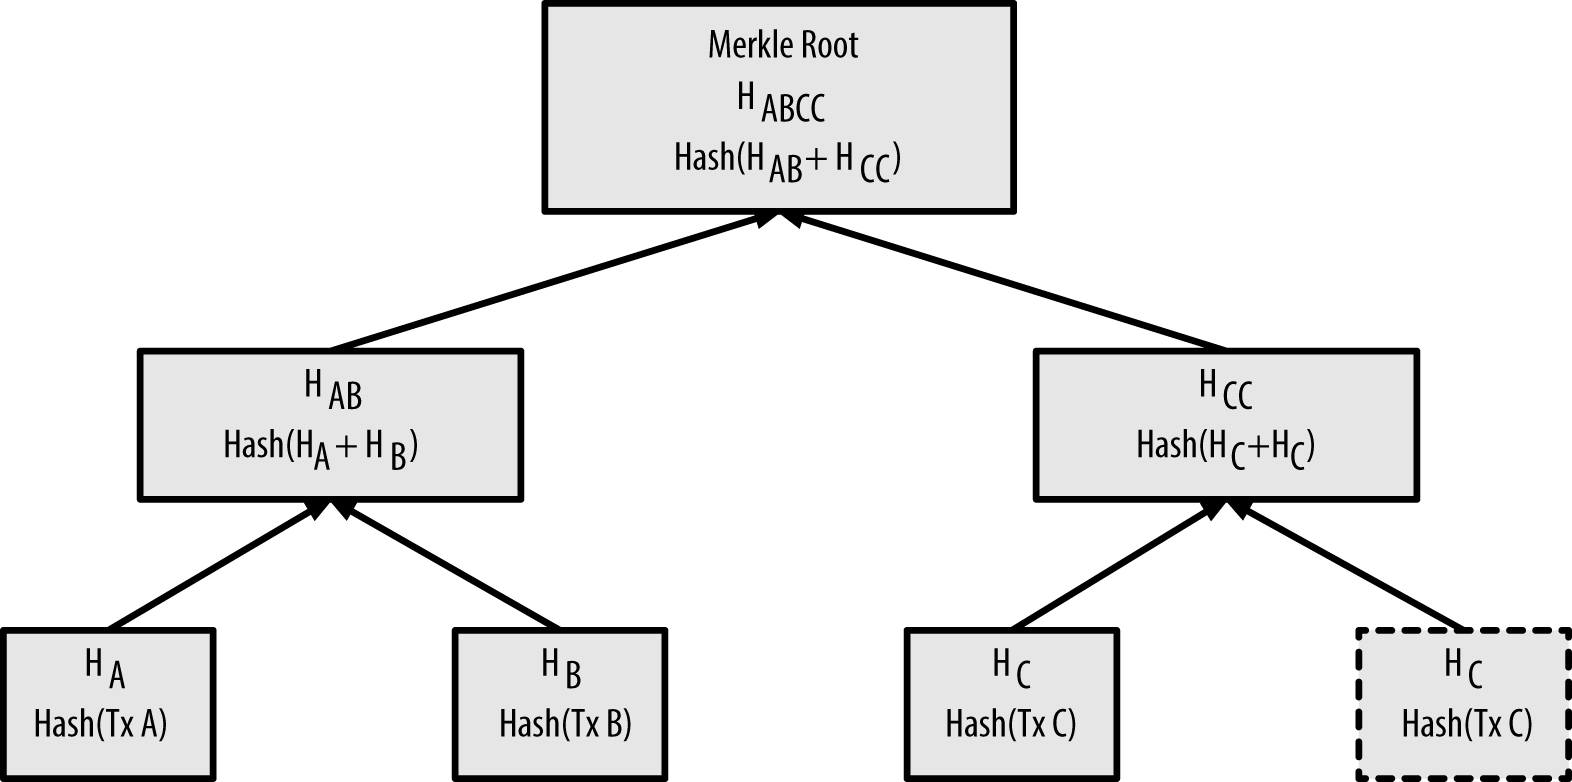
\includegraphics[scale=1.0]{images/merkle_tree.png}
	\caption{Node hashes in a  merkle tree \citep{bitcoin}}
	\label{fig:merkle_tree}
\end{figure}

With this the application can tell if there is any change in the current section of the tree just by comparing the nodes hashes without having to loop over them, allowing the program to only loop over the nodes when a change is detected. Allowing it to skip the parts that have not been changed. Unless the entire database is modified where the application will have to revert to looping over everything. The hash for each node is calculated off the hash of the data inside it, and its children's data. This will let the application detect if a page has been added, removed or modified. 
\\\\
When the application detects an update to the data, it will mark that page as modified, a simple boolean value. Recording the string value, from the old page and new page, into a log object. If instead it was a removal or addition, of data, it will store the new / removed value. Something similar happens with added and removed pages. With the addition of pages, the added page will be marked as changed. Often when this happens a pointer to the new page will also be placed somewhere, so this is also recorded. When a  page is removed, utilising the data from the old tree allows the application to see exactly what was page has been removed and can record it, but there is nothing to marked as changed, since it no longer exists, apart from the pointers in other pages to that page. 

\subsubsection{Live Updater}
\label{subsubsec:live_Updater_imp}

The Live updater has undergone many changes from the start, although its position in the architecture has not changed, it gradually was morphed and shaped by the rest of the application. Originally the live updater started out as a module that would control the parsing of the application. By contacting the database and telling it when to move along the time line, allowing the pausing of live updates. It would also receive the update signal from the file watcher, and parse the file, moving it into the database storage. Basically an extra more controlled, and tailored interface into the database interface linking it to the file parser.
\\\\
However, to collect metadata information about the database, the live updater had to run SQL onto the database, else it would have to loop through the entire tree again. So it needed access to the SQL executer, which is covered in the next section. Then the problems with the logging came up, and while working a way around these problem, it ended up inside of the live updater. As a result of this the module soon became bloated, as new features were added since this was the only module that had access to all the needed resources.
\\\\
Rather than fighting against the application design, it would be better to dedicate this as a sort of master module, that would orchestrate the process when an update signal is revived. This allowed the extra tasks that where piled on to move on back into their correct modules, as a result of this it does exactly what was set out in the beginning. Acting as a tailored interface into the database interface, contacting the file parser, SQL executor, and Log modules to control the parsing of the updated database.
\\\\
When an update signal is received, the live updater requests a database object from the file parser, and adds the extra metadata from the SQL command. It then requests the previous database object from the database interface, and sends them to the log. Before storing the new database object inside the database interface. If the application is not paused it will then increment along the time line. 

\subsubsection{SQL executor}
\label{subsubsec:sql_executor_imp}

The SQL executor manages the JDBC connections to the database, making sure that it connects, closes and commits any changes that are needed onto the database. Its interface provides five methods to the other modules, connect, close, perform select, perform update and get database metadata. Unlike the rest of the modules this was one of the more straight forward and simple to implement, calling the corresponding functions on the JDBC API.

\subsection{User Interface}
\label{subsec:user_interface_imp}

The last section mentioned how the view is put together, but now that each of the modules have been looked at in turn. This section will go through how each of the different tabs / features are put together. In order to better understand how each module is interacted with.
\\\\
The entire user interface is made up of eight FXML files and one CSS file, for styling. As mentioned previously, the FXML files contain the layout for each of the sections. Therefore  each of the sections seen by the user represents a single FXML file. The application takes on a dark colour scheme used throughout, due to personal preference, however this could easily be swapped out for a lighter color scheme. 
\\\\
The menu bar is made up of one FXML file. In addition to the visual elements using the JavaFX key code combination class it provides keyboard short-cuts, such as `control o' to open a database, and `control-q' to quit. The controller for this FXML file  contacts the model interface for the opening and closing the database, and the live updater for controlling the timeline.  This can be seen below in figure~\ref{fig:ui_screen}.

\begin{figure}[H]
	\centering
	
\includegraphics[scale=0.32]{images/ui_screen.png}
	\caption{Menu bar.}
	\label{fig:ui_screen}
\end{figure}

The right section is made up of a single FXML file, containing the SQL executer. As previously mentioned the SQL executor module enables arbitrary SQL commands to be ran on the database. As such this section contacts the SQL executor in order connect, run commands, and close the connection. The final interface can be seen below in figure~\ref{fig:ui_imp_sqlexe}.

\begin{figure}[H]
	\centering
	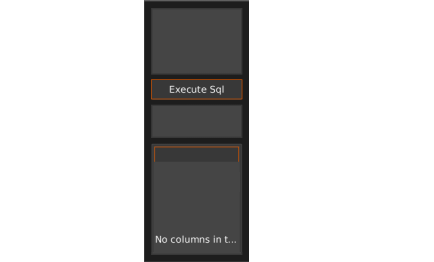
\includegraphics[scale=0.7]{images/ui_sqlexe_design_final.png}
	\caption{SQL executor UI.}
	\label{fig:ui_imp_sqlexe}
\end{figure}

The metadata tab is made up of single FXML file. The outer layer is a scroll pane, with a flow pane content. The flow pane provides a dynamic layout to adjust to different resolutions alongside the scroll pane. The panels, inside of the flow pane are panes with grid pane content. The grid pane has two columns. The left or first column, representing the description or name and the right or second column the value. In order to collect the metadata, the controller needs to contact the database interface, to collect the current database object. The user interface can be seen below in figure~\ref{fig:ui_imp_metdata}.

\begin{figure}[H]
	\centering
	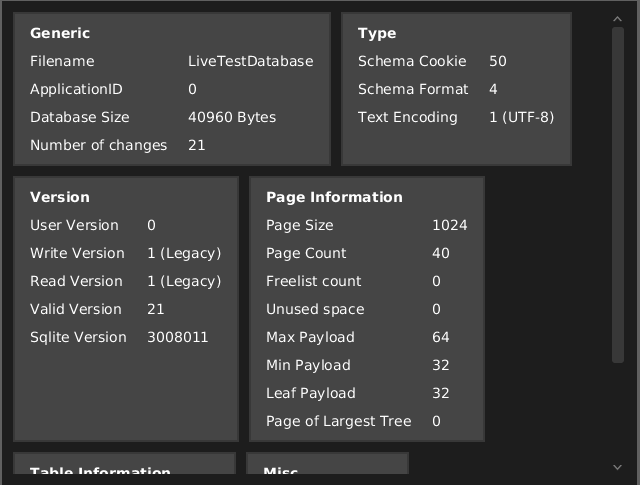
\includegraphics[scale=0.32]{images/ui_meatadata_final.png}
	\caption{Metadata UI.}
	\label{fig:ui_imp_metdata}
\end{figure}

The table view is made up of two FXML files that share a controller. The table view allows users to select a  table and view the schema and all the data within it. In order to accomplish this it contacts the SQL executor, and runs a select all query to collect the data, and a select from `sqlite\verb|_|master' to retrieve all tables and schemas. This interface can be seen below in figure~\ref{fig:imp_ui_table}.

\begin{figure}[H]
	\centering
	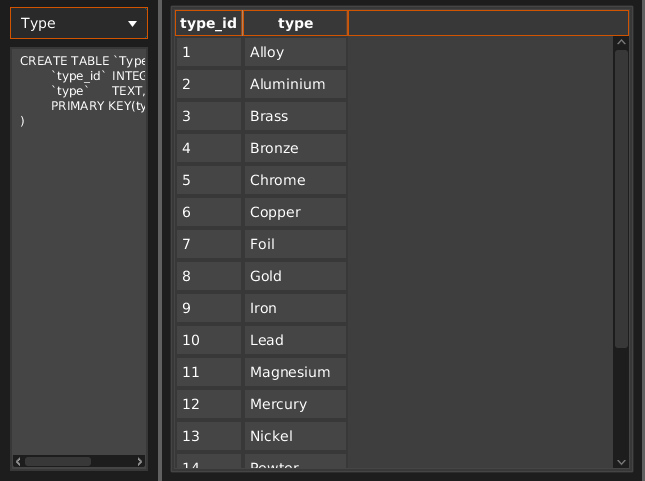
\includegraphics[scale=0.32]{images/ui_table_final.png}
	\caption{Table view UI.}
	\label{fig:imp_ui_table}
\end{figure}

The visualiser is made up of two FXML files, sharing a single controller. The centre section containing the visualisation of the database, uses a custom scroll pane node to enable, zooming in addition to scrolling. Each node is represented as a pane, with a CSS class for the colouring. The node, contains the corresponding B-Tree node, from the database object. This is then used to display the data within the left side pane. In order to draw the structure the first pass sorts out the horizontal position going top down. This is also used to load the nodes, via recursion. After all the nodes are loaded a second pass is used to then calculate the horizontal positions using a bottom up approach. This interface can be seen below in figure~\ref{fig:imp_ui_vis}.

\begin{figure}[H]
	\centering
	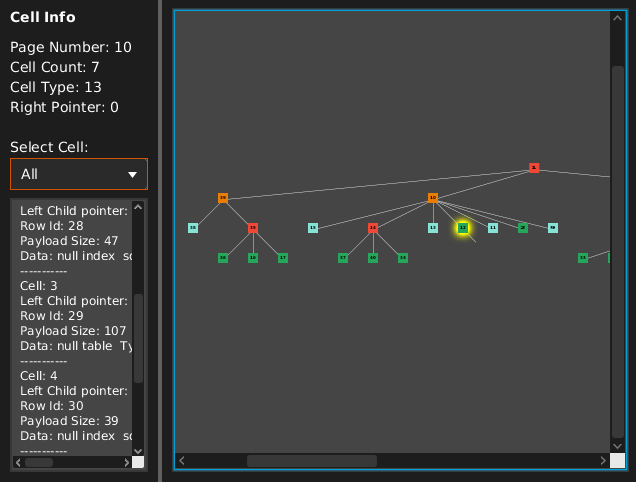
\includegraphics[scale=0.32]{images/ui_visuliser_final.png}
	\caption{Visualiser interface design.}
	\label{fig:imp_ui_vis}
\end{figure}

The log is made up of one FXML file. Similar to the metadata tab, it contains a single scroll pane, with a VBox inside, allowing it to contain infinite items. Each item is made up of a Titled pane. Where the title is the time and data of the update, and the content, the changes that where performed in the update. To collect the data, it contacts the Log module, and receives a list of log items. This can be seen below in figure~\ref{fig:imp_ui_log}.

\begin{figure}[H]
	\centering
	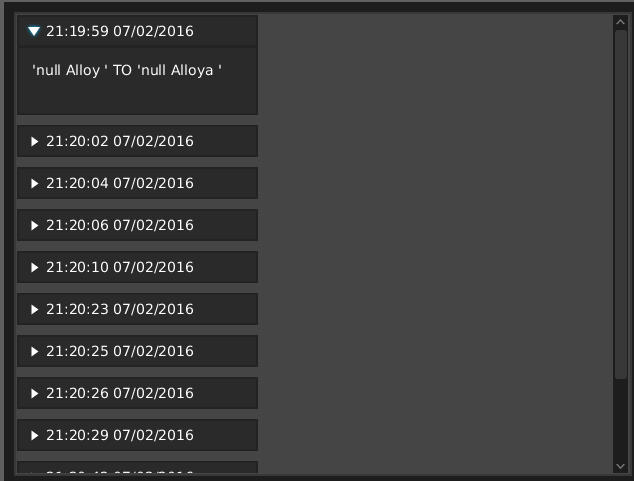
\includegraphics[scale=0.32]{images/ui_log_final.png}
	\caption{Log UI.}
	\label{fig:imp_ui_log}
\end{figure}

	\section{System Operation}
\label{sec:system_operation}
	\section{Testing}
\label{sec:testing}

Testing is an important part of making all application, and as such will go over the ways that I went about testing my application.

\subsection{Test data}
\label{subsec:test_data}

In order to assure that my program ran correctly under a variety of circumstances, I used a variety of databases including different sizes, and headers. 

\subsection{Unit tests}
\label{subsec:unit_tests}

Throughout the implementation stage I kept close to test driven development, and as such have written a lot of unit tests utilising the JGroups framework. In total I have around TODO:X unit tests. All passing. The unit tests are written to use mocks where dependences are needed allowing me to make sure its correctly testing.
\\\\
In order to test the user interface I found a test framework that works alongside called testFx that is specifically designed to test JavaFX. You pass it the root node of your scene, and pass it commands, such as click, with either the id, or name of the item. It will then automatically control the mouse, interacting with the user interface.

\subsection{Integration tests}
\label{subsec:integration_tests}

In addition to unit testing, I performed integration tests that would test the interactions between the various modules in order to check that they are working correctly. Such as the live updater and it corresponding calls to the other modules. This also included testing that the user interface would correctly interact with the module and its various modules correctly.

\subsection{Manual testing}
\label{subsec:mamual_tests}

Where such tests needed a a human eye, such as the design and drawing of items, and other small interactions that could not be automated. I manually over saw theses test. However, the majority of manual testing, were small things that would not affect the application to any great affect.
	\section{Evaluation}
\label{sec:evaluation}

In this section we will reflect on the final results from this project, and whether we have met our overall aims. And the design principles used through the undertaking of the project.

\subsection{Design principles}
\label{subsec:design_principles}

Through the project I tried to keep as close to good OOP paradigms and design as possible. Creating a effective tool that anyone could use. As stated in the introduction the main was to build tool that anyone could use to debug their own databases, with the five main features visualisation, live updating, executing SQL and browsing data. Wrapped up within a user interface. 
\\\\
With support for other database system when needed, just by extending the interfaces and providing an implementation. In addition to sticking to good OPP design, I used TDD ( Test driven development ) in order to make sure that the final application, would work under a variety of circumstances. In the end I can safely say they theses aims where achieved. With the exception, of the lock byte and pointer map pages. 

\subsection{The System}
\label{subsec:system_eval}

The application its self though built in Java does not have many performance hiccups or other issues. 
\\\\
TODO: TALK ABOUT SYSTEM PERFORMANCE, HOW LONG IT TAKE TO PARSE THE DATABASE.

\subsection{User interface}
\label{subsec:user_interface_eval}

TODO EVAL THE USER INTERFACE DESIGN WHEN FINISHED.
	%
% The MIT License (MIT)
%
% Copyright (c) 2016 Paul Batty
%
% Permission is hereby granted, free of charge, to any person obtaining a copy
% of this software and associated documentation files (the "Software"), to deal
% in the Software without restriction, including without limitation the rights
% to use, copy, modify, merge, publish, distribute, sublicense, and/or sell
% copies of the Software, and to permit persons to whom the Software is
% furnished to do so, subject to the following conditions:
%
% The above copyright notice and this permission notice shall be included in
% all copies or substantial portions of the Software.
%
% THE SOFTWARE IS PROVIDED "AS IS", WITHOUT WARRANTY OF ANY KIND, EXPRESS OR
% IMPLIED, INCLUDING BUT NOT LIMITED TO THE WARRANTIES OF MERCHANTABILITY,
% FITNESS FOR A PARTICULAR PURPOSE AND NONINFRINGEMENT. IN NO EVENT SHALL THE
% AUTHORS OR COPYRIGHT HOLDERS BE LIABLE FOR ANY CLAIM, DAMAGES OR OTHER
% LIABILITY, WHETHER IN AN ACTION OF CONTRACT, TORT OR OTHERWISE, ARISING FROM,
% OUT OF OR IN CONNECTION WITH THE SOFTWARE OR THE USE OR OTHER DEALINGS IN
% THE SOFTWARE.
%

\section{Conclusion}
\label{sec:conclusion}

The start of this paper defined some very clear goals that this project hoped to achieve by the end of it. Firstly, to understand of why SQLite is so good, what makes it so prevalent and how it works. This included the file format and its systems. This was achieved throughout the first chapter of this paper. 
\\\\
The second aim was to take this knowledge and build a tool that could record all operations performed onto the database. While providing the same insight gathered throughout this project without having to look through a Hex editor. It should also be easy to use and well tested. Making it reliable and efficient. This was successfully achieved through the second to forth sections.
\\\\
Lastly, to look at where this project could be taken in the future, and what could be done to take the application to the next stage. This involved critically evaluating the final application and what could be changed or added. This was achieved in the final sections of this paper.
\\\\
In conclusion this project has been an overall success. The main aims that have been set out were reached. However, the performance could still be improved. The user interface stills need some polishing in order to make it more user friendly. Providing a better visualisation of the database. Though the last stretch is always the longest and a lot of time could be spent polishing the interface, and fixing all the edge cases that have not yet made themselves apparent.
\\\\
In the future, other features could be added such as providing support for the other system such as  extensions, lock byte and pointer map pages, and any other changes made to SQLite. Another project that would also be useful stemming off of this one is to try and recreate the original SQL query sent to the database based on the changes made, since it can only currently only list the changes. 
\\\\
But, with that said this has been an enjoyable project, and by then end of it all have learnt a great deal about SQLite, Java and JavaFX, some more of the unique data structures such as the Merkle trees. In addition to a nice tool that can be used in the future whenever working on a SQLite database to discover any problems.
	\section{References}
\label{sec:references}

\bibliography{sqlite_visualiser_report.bib}	

\begin{thebibliography}{0}

% order aphabeticaly by first name.
\bibitem[Sotomayor, 2010]{chibd}
Sotomayor B. (2010), The xdb File Format. On line publication, University of Chicago, http://people.cs.uchicago.edu/\verb|~|borja/chidb/chidb\verb|_|fileformat.pdf. Last Accessed 18th January 2016.

\bibitem[Comer, 1979]{btreepaper}
Comer D. (1979) Towards Computing Surveys. The Ubiquitous B-Tree, Computing Surveys, Vol 11, No. 2. Purdue University, West Lafayette, Indiana, June 1979, pages 121 - 137.

\bibitem[Knuth, 1973]{btreeimprpaper}
Knuth E. D. (1973) The Art Of Computer Programming, Volume 3: "Sorting And Searching", Addison-Wesley Publishing Company, Reading, Massachusetts. Pages 473 - 480.

\bibitem[Owens, 2006]{sqlitedefguide} 
Owens M. (2006). The Definitive Guide to SQLite, Berkeley, California, Apress. 

\bibitem[Hipp, 2000]{sqlite} 
Hipp R. (2000) Sqlite. On line publication, Wyrick Company, Inc, https://www.sqlite.org/. Last Accessed 17th January 2016.

\bibitem[Hipp, 2015]{sqlitetalk} 
Hipp R. (2015) SQLite: The Database at the Edge of the Network. On line Video, Skookum, https://www.youtube.com/watch?v=Jib2AmRb\verb|_|rk. Last Accessed 17th January 2016.

\bibitem[Drinkwater, 2011]{sausagefactory}
Drinkwater R. (2011) An analysis of the record structure within SQLite databases, Forensics from the sausage factory, On line publication, http://forensicsfromthesausagefactory.blogspot.com/2011/05/analysis-of-record- \newline structure-within.html, Last Accessed 17th January 2016.

\bibitem[Raymond, 2009]{sqliteray}
Raymond, (2009) SQlite.  On line publication, http://ray.bsdart.org/man/sqlite/. Last Accessed 17th January 2016.

\end{thebibliography}
	%
% The MIT License (MIT)
%
% Copyright (c) 2016 Paul Batty
%
% Permission is hereby granted, free of charge, to any person obtaining a copy
% of this software and associated documentation files (the "Software"), to deal
% in the Software without restriction, including without limitation the rights
% to use, copy, modify, merge, publish, distribute, sublicense, and/or sell
% copies of the Software, and to permit persons to whom the Software is
% furnished to do so, subject to the following conditions:
%
% The above copyright notice and this permission notice shall be included in
% all copies or substantial portions of the Software.
%
% THE SOFTWARE IS PROVIDED "AS IS", WITHOUT WARRANTY OF ANY KIND, EXPRESS OR
% IMPLIED, INCLUDING BUT NOT LIMITED TO THE WARRANTIES OF MERCHANTABILITY,
% FITNESS FOR A PARTICULAR PURPOSE AND NONINFRINGEMENT. IN NO EVENT SHALL THE
% AUTHORS OR COPYRIGHT HOLDERS BE LIABLE FOR ANY CLAIM, DAMAGES OR OTHER
% LIABILITY, WHETHER IN AN ACTION OF CONTRACT, TORT OR OTHERWISE, ARISING FROM,
% OUT OF OR IN CONNECTION WITH THE SOFTWARE OR THE USE OR OTHER DEALINGS IN
% THE SOFTWARE.
%

\section{Appendix}
\label{sec:appendix}

\subsection{Appendix A}
\label{subsec:append_a}

Table~\ref{tbl:sqlite_header} show the header layout.  All multibyte fields are stored in a big-endian format.

\begin{longtable}[h]{| c | c | p{10cm} |}
		\hline
			\textbf{Byte Offset} & \textbf{Byte Size} & \textbf{Description} \\ 
		\hline
		\endhead
			0 & 16 & A UTF-8 Header String followed by null terminator read as: "SQLite format 3" or in hex: "53 51 4c 69 74 65 20 66 6f 72 6d 61 74 20 33 00". \\
		\hline
			16 & 2 & Page Size 	in bytes, power of two between 512 - 65536 bytes. if using version 3.7.0.1 and earlier between 512 - 32768, or 1 for 65536. \\
		\hline
			18 & 1 & Write version, 1 for legacy; 2 for WAL. \\
		\hline
			19 & 1 & Read version, 1 for legacy; 2 for WAL. \\
		\hline
			20 & 1 & Bytes of unused space at the end of each page. This space is used by extensions, such as cryptographic to store a checksum, but normally 0. \\
		\hline
			21 & 1 & Maximum embedded payload fraction, must be 64. Was going to be used to determine the maximum size of a B-Tree cell on a index B-Tree. \\
		\hline
			22 & 1 & Minimum embedded payload fraction, must be 32. Was going to be used to determine the portion of a B-Tree cell that has one or more overflow pages on a index B-tree. \\
		\hline
			23 & 1 & Leaf payload fraction, must be 32. Was going to be used to determine the portion of a B-Tree cell that has one or more overflow pages on a leaf or table B-Tree. \\
		\hline
			24 & 4 & File change counter. It counts the number of times the database is unlocked after being modified. May not be incremented in WAL mode. \\
		\hline
			28 & 4 & Size of the database in pages, Total number of pages. \\
		\hline
			32 & 4 & Page number of first freelist page, or 0 if no freelist. \\
		\hline
			36 & 4 & Number of freelist pages. \\
		\hline
			40 & 4 & Schema Cookie. The schema version, each time the schema is modified this number is incremented. \\
		\hline
			44 & 4 & Schema format number. either 1, 2, 3 or 4. \newline
			1. Format support back to version 3.0.0. \newline
			2. Varying number of columns within the same table. From Version 3.1.3. \newline 
			3. Extra column can be non-NULL values. From Version 3.1.4. \newline
			4. Respects DESC keyword and boolean type. From Version 3.3.0. \newline \\
		\hline
			48 & 4 & Page cache size. suggestion only towards Sqlite's pager. \\
		\hline
			52 & 4 & Page number of largest root B-Tree, when in vacuum mode else 0. \\
		\hline
			56 & 4 & Text encoding. \newline
			 1 for UTF-8. \newline 
			 2 for UTF-816le. \newline 
			 3 for UTF-816be. \\
		\hline
			60 & 4 & User version. Set by and read by the user, not used by Sqlite. \\
		\hline
			64 & 4 & Incremental-vacuum mode. Non 0 for true. 0 for false \\
		\hline
			68 & 4 & Application ID. Used to associate the database with a application. 0 is Sqlite3 Database \\
		\hline
			72 & 20 & Empty, Reserved for expansion. \\
		\hline
			92 & 4 & Version-valid-for-number. Value of the change counter when the Sqlite version number was stored. \\
		\hline
			96 & 4 & Version. Sqlite version. \\
		\hline
	\caption{Sqlite Header, modified from \cite{sqlite}}
	\label{tbl:sqlite_header}
\end{longtable}

\subsection{Appendix B}
\label{subsec:append_b}

Time in milliseconds to parse a database.

\begin{longtable}[h]{| c |}
		\hline
			\textbf{Time in milliseconds} \\ 
		\hline
		\endhead
 		210 \\
 				\hline
		147 \\
				\hline
		147 \\
				\hline
		163 \\
				\hline
		145 \\
				\hline
		142 \\
				\hline
		141 \\
				\hline
		139 \\
				\hline
		138 \\
				\hline
		169 \\
				\hline
	\caption{Time in miliseconds to parse}
	\label{tbl:time_patse}
\end{longtable}

\section{Code}
\subsection{More code}
\subsubsection{Even more code}
This is some very important code.
This is a very long sentance in order to see hoow latex copes with very very long lines of non stop text.
\begin{lstlisting}
	// main
	public static void main(String args[]) {
		System.out.println("Hello World");
	}
\end{lstlisting}

And so on..

\end{document}